\documentclass[a4paper,11pt, DIV=11]{scrartcl}
\usepackage{amsmath,amsthm}
\usepackage{csquotes}
\usepackage{anyfontsize}
\usepackage{a4wide}
\usepackage[type1,sb]{libertine}
\usepackage[libertine]{newtxmath}
\usepackage{inconsolata}
\usepackage[scr=rsfso]{mathalfa}
\usepackage[UKenglish]{babel}
\usepackage{microtype}
\usepackage{interval}
\intervalconfig{soft open fences}
\usepackage{thm-restate}
\usepackage{complexity}
\usepackage{comment}
\usepackage{hyperref} 
\usepackage{xcolor}

\definecolor{myBlue}{RGB}{27, 82, 140}
\definecolor{myBrightBlue}{RGB}{24, 107, 196}
\definecolor{myGreen}{RGB}{82, 140, 27}
\definecolor{myBrightGreen}{RGB}{107, 196, 24}
\definecolor{myRed}{RGB}{140, 27, 82}
\definecolor{myBrightRed}{RGB}{196, 24, 107}

\hypersetup{colorlinks,allcolors=myBlue}

\usepackage{todonotes} 
\usepackage{optidef} 
\usepackage{tikz}
\usepackage{pgfplots}
\usetikzlibrary{calc}
\usepackage[nameinlink]{cleveref}
\usepackage{bm}
\usepackage{enumitem}

\newcommand\B[1]{{\textstyle\binom{#1}{\lfloor #1/2 \rfloor}}}
\newcommand{\vx}{\ensuremath{\mathbf{x}}}
\newcommand{\vy}{\ensuremath{\mathbf{y}}}
\newcommand{\vb}{\ensuremath{\mathbf{b}}}
\newcommand{\va}{\ensuremath{\mathbf{a}}}



\hyphenation{non-ap-prox-i-ma-bi-li-ty}

\renewcommand{\epsilon}{\varepsilon}
\renewcommand{\phi}{\varphi}

\newcommand{\ignore}[1]{}

\newlist{algoEnum}{enumerate}{10}
\setlist[algoEnum, 1]{label={\arabic*.}}
\setlist[algoEnum, 2]{label={(\roman*)}}

\creflabelformat{algoEnumi}{#2#1#3}
\creflabelformat{algoEnumii}{#2#1#3}

\crefname{algoEnumi}{step}{steps}
\crefname{algoEnumii}{case}{cases}

\pgfplotsset{compat=1.18}
\usepgfplotslibrary{fillbetween}
\usetikzlibrary{calc}
\usetikzlibrary{patterns}


\renewcommand{\G}{\ensuremath{\mathfrak{G}}}

\DeclareMathOperator{\NBin}{NBin}
\DeclareMathOperator{\id}{id}
\DeclareMathOperator{\elin}{\textnormal{\textsf{E3Lin}}}
\DeclareMathOperator{\belin}{\textnormal{\textsf{BalancedE3Lin}}}

\DeclareMathOperator{\maxPCSP}{\textup{MaxPCSP}}

\DeclareMathOperator{\maxCSP}{\textup{MaxCSP}}

\DeclareMathOperator{\CSP}{\textup{CSP}}
\DeclareMathOperator{\PCSP}{\textup{PCSP}}

\newcommand{\N}{\ensuremath{\mathbb{N}}}
\renewcommand{\R}{\ensuremath{\mathbb{R}}}

\theoremstyle{plain}
\declaretheorem[shaded={bgcolor=myBlue!5}]{theorem}
\declaretheorem[sibling=theorem, shaded={bgcolor=myBlue!5}]{lemma, proposition, corollary, conjecture}

\theoremstyle{definition}
\declaretheorem[sibling=theorem, shaded={bgcolor=myBlue!5}]{definition}

\usepackage{marginnote}

\newcommand{\SZ}[1]{{\color{red}\marginnote{\textbf{SZ}:#1}}}
\newcommand{\TVN}[1]{{\color{blue}\marginnote{\textbf{TVN}:#1}}}

\newclass\UGC{UGC}

\setkomafont{author}{\normalfont\large}
\setkomafont{date}{\normalfont\large}

\begin{document}

\title{A Dichotomy for Maximum PCSPs on Graphs\thanks{An extended abstract of a part of this work will appear in Proceedings of ICALP\,(A) 2025. This work was supported by UKRI EP/X024431/1 and Clarendon Fund Scholarship. For the purpose of Open Access, the authors have applied a CC BY public copyright licence to any Author Accepted Manuscript version arising from this submission. All data is provided in full in the results section of this paper.}}

\author{Tamio-Vesa Nakajima\\
University of Oxford\\
\url{tamio-vesa.nakajima@cs.ox.ac.uk}
\and
Stanislav \v{Z}ivn\'y\\
University of Oxford\\
\url{standa.zivny@cs.ox.ac.uk}
}

\date{} 

\maketitle


\begin{abstract}
Fix two non-empty loopless graphs $G$ and $H$ such that $G$ maps homomorphically to $H$. The \emph{Maximum Promise Constraint Satisfaction Problem} parameterised by $G$ and $H$ is the following computational problem, denoted by $\maxPCSP(G, H)$: Given an input (multi)graph $X$ that admits a map to $G$ preserving a $\rho$-fraction of the edges, find a map from $X$ to $H$ that preserves a $\rho$-fraction of the edges. As our main result, we give a complete classification of this problem under Khot's Unique Games Conjecture: The only tractable cases are when $G$ is bipartite and $H$ contains a triangle. 

Along the way, we establish several results, including an efficient approximation algorithm for the following problem: Given a (multi)graph $X$ which contains a bipartite subgraph with $\rho$ edges, what is the largest triangle-free subgraph of $X$ that can be found efficiently? We present an SDP-based algorithm that finds one with at least $0.8823 \rho$ edges, thus improving on the subgraph with $0.878 \rho$ edges  obtained by the classic Max-Cut algorithm of Goemans and Williamson.

\end{abstract}


\section{Introduction}

Given two undirected graphs\footnote{All graphs in this article are loopless and
non-empty, meaning having at least one edge (and thus at least two vertices).}
$G$ and $H$, a \emph{homomorphism} from $G$ to $H$ is an edge preserving map $h$
from $V(G)$ to $V(H)$; that is, if $(u,v)\in E(G)$ then $(h(u),h(v))\in
E(H)$. A classic result of Hell and Ne\v{s}et\v{r}il established a computational
\emph{dichotomy} for the so-called $H$-colouring
problem~\cite{Hell90:h-coloring}, for a fixed graph $H$: if $H$ is bipartite then deciding whether an
input graph $G$ is homomorphic to $H$ is solvable in polynomial time, and for
every other $H$ this problem is NP-complete. Going beyond graphs, Feder and
Vardi conjectured that a similar dichotomy holds for all finite relational
structures~\cite{FederVardiConjecture}, not only for graphs and for relational structures over
the Boolean domain~\cite{Schaefer78:stoc}.\footnote{We will not need relational
structures, but, intuitively, one should think of them as generalisations of
(hyper)graphs in which one is given a ground set and a collection of relations
on the ground set.} Bulatov~\cite{Bulatov17:focs} and, independently,
Zhuk~\cite{Zhuk20:jacm}, confirmed the tractability part of the dichotomy, which
together with the NP-hardness part~\cite{Bulatov05:classifying}, answered the
Feder-Vardi conjecture in the affirmative. The homomorphism problem is also
known as the \emph{constraint satisfaction problem} (CSP)~\cite{Jeavons98:algebraic}. CSPs can be
equivalently defined as problems seeking an assignment of values to the
given variables subject to the given constraints. The fixed target structure in
the homomorphism problem corresponds to the set of allowed (domain) values and
the set of allowed relations in the constraints. Concrete examples of CSPs include
solvability of linear equations over finite fields and variants of (hyper)graph
colourings.

A well-studied line of work focuses on \emph{approximability} of
CSPs~\cite{KSTW00,Trevisan00:sicomp}. A classic example here is
the Max-Cut problem. In Max-Cut, the variables correspond to the
vertices of the input graph, the values are just $0$ and $1$ (corresponding to
the two sides of a cut), and the constraints are binary disequalities associated
with the edges of the graph. Given a CSP, the computational task could be to
find a solution maximising the number of satisfied constraints as in Max-Cut, or
finding a (perfect) solution satisfying all constraints as discussed in the
previous paragraph. 

A \emph{promise} CSP (PCSP) is a CSP in which each
constraint comes in two forms, a strong one and a weak one. The promise is that
a solution exists using the strong versions of the constraints, while the
(possibly easier) task is to find a solution using the weak constraints. A
recent line of work by Austrin, Guruswami, and H{\aa}stad~\cite{AGH17},
Brakensiek and Guruswami~\cite{BG21:sicomp}, and Barto, Bul\'in, Krokhin, and
Opr\v{s}al~\cite{BBKO21} initiated a systematic study of PCSPs with perfect completeness,
i.e., finding a solution satisfying all weak constraints given the promise that
a solution satisfying all strong constraints exists. Canonical examples include 
approximate graph~\cite{GJ76} and hypergraph~\cite{DRS05,ABP20,Barto21:stacs} colouring problems,
e.g., finding a 5-colouring of a given 3-colourable graph~\cite{KOWZ23}.
PCSPs are a vast generalisation of CSPs and their complexity is not well
understood, not even on the Boolean domain~\cite{Ficak19:icalp,BGS23} or for
graphs. In particular, Brakensiek and Guruswami conjectured that only bipartite
graphs lead to tractable PCSPs on graphs~\cite{BG21:sicomp} (cf.~\Cref{conjBG}
in~\Cref{sec:results} for a precise statement). Resolving their 
conjecture would in particular include resolving the notoriously difficult approximate graph
colouring problem, cf.~\cite{Avvakumo25:stoc} for exciting recent progress.

\medskip

In this work, we will focus on the \emph{approximability of maximisation PCSPs}. The ultimate goal is to understand the precise
approximation factor for all $\maxPCSP$s, and thus identify where the transition
from tractability to intractability occurs. This is an ambitious, long-term goal
that would encompass many existing fundamental results.

An example of a $\maxPCSP$ is the following problem. Given a graph $G$ that
admits a $2$-colouring of the vertices with a $\rho$-fraction of the edges
coloured properly, find a $3$-colouring of $G$ with an $\alpha\rho$-fraction of
the edges coloured properly, where $0<\alpha\leq 1$ is the approximation factor.
As one of the results in the present paper, we will show that there is a
1-approximation algorithm; i.e., given a graph with a 2-colouring with
$\rho$-fraction of non-monochromatic edges, one can efficiently find a
3-colouring of the graph with the same fraction of non-monochromatic edges. 

As our main result, we will establish a dichotomy for 1-approximation of graph
PCSPs under Khot's Unique Games Conjecture (\UGC)~\cite{Khot02stoc}.

\begin{restatable}{theorem}{UGCdichotomy}\label{thm:UGCdichotomy}
  Let $G$ and $H$ be two fixed graphs such that there is a homomorphism from $G$ to $H$. 
  If $G$ is bipartite and $H$ contains a triangle then $\maxPCSP(G,H)$ is 1-approximable. Otherwise, 1-approximation of $\maxPCSP(G,H)$ is \NP-hard assuming the \UGC.
\end{restatable}

Along the way to prove~\Cref{thm:UGCdichotomy}, we will design two efficient
approximation algorithms. We shall discuss one of them briefly here, with an
overview of both algorithms and all results in~\Cref{sec:results}.

Given an undirected (multi)graph $G$, what is the bipartite subgraph of $G$ with
the most edges? This is nothing but the already mentioned Max-Cut problem, one of the most fundamental problems in computer science.
Max-Cut was among the 21 problems shown to be \NP-hard by Karp~\cite{Karp1972}.
Papadimitriou and Yannakakis showed that Max-Cut is
\APX-hard~\cite{PapadimitriouY91} and thus does not admit a polynomial-time
approximation scheme, unless $\P=\NP$. However, there are several simple
$0.5$-approximation algorithms. Goemans and Williamson used semidefinite
programming and randomised rounding to design a $0.878$-approximation
algorithm~\cite{GW95}. 
Khot, Kindler, Mossel, O'Donnell, and Oleszkiewicz established the optimality of
this algorithm~\cite{KKMO07,Mossel10:ann} under the \UGC.

\begin{center}\emph{What if the task is merely finding a large
  \underline{triangle-free} subgraph (rather than a bipartite one)?}
\end{center}

While the Goemans-Williamson algorithm can still be used, as one of our results
we design an algorithm with a better approximation guarantee: If $G$ contains a
bipartite subgraph with $\rho$ edges, our algorithm efficiently finds a
triangle-free subgraph of $G$ with $0.8823\rho$ edges.\footnote{We note that our
algorithm is easy to extend to the case where edges have positive weights.} Our
algorithm is a randomised combination of the Goemans-Williamson original
``random hyperplane algorithm'', and an algorithm that first selects ``long
edges'' (meaning edges for which the angle between the corresponding vectors
from the SDP solution is above a certain threshold) and then applies a random
hyperplane rounding, selecting ``shorter edges'' (still longer than some other
threshold). The probability of the biased coin that selects one of the two
algorithms depends on certain geometric quantities which guarantee that the
resulting subgraph is indeed triangle-free.
We complement our tractability result for this problem by showing that it is
$\NP$-hard to find a triangle-free subgraph with $(25 / 26 + \epsilon) \rho
\approx (0.961 + \epsilon) \rho$ edges. This result is obtained by a reduction
from H\aa{}stad's 3-bit PCP~\cite{Hastad01}.


\paragraph{Related work}

The notion of $\maxPCSP$s is a natural generalisation of the well-studied notion of $\maxCSP$s. 
For finite-domain $\maxCSP$s, it is known that a certain rounding of the basic SDP relaxation gives,
up to some $\epsilon$,
the \UGC-optimal approximation ratio (in time doubly exponential in $1 /
\epsilon$)~\cite{Raghavendra08:everycsp,Raghavendra09:focs}. 
However, the
Raghavendra-Steurer algorithm does not immediately give a 1-approximation
algorithm due to the above-mentioned $\epsilon$, even for $\maxCSP$s. Moreover,
that result is established only for finite-domain $\maxCSP$s. 
On other hand, our results include a 1-approximation for $\maxPCSP(K_2,
K_3)$, and an algorithm for infinite-domain structures, namely for
$\maxPCSP(K_2, \G_3)$, which captures the bipartite vs. triangle-free subgraph
discussed above (cf.~\Cref{sec:prelims} for a precise definition).

Approximation of concrete $\maxPCSP$s has been studied for decades, include
several papers on almost approximate graph
colouring~\cite{Engebretsen08:rsa,Dinur10:focs,Khot12:focs,Hecht23:approx},
approximate colouring~\cite{nz23:arxiv}, and promise
Max-3-LIN~\cite{blz25:icalp}. Our work initiates a systematic investigation,
giving a complete classification for 1-approximation of the graph case.

Recent work of Brakensiek, Guruswami, and Sandeep~\cite{BGS23:stoc} studied
robust approximation of $\maxPCSP$s; in particular, they state that
Raghavendra's above-mentioned theorem on approximate
$\maxCSP$s~\cite{Raghavendra08:everycsp} applies verbatim to $\maxPCSP$s. This
in combination with the work of Brown-Cohen and Raghavendra~\cite{BCR15} gives a
framework for studying approximation of $\maxPCSP$s. An alternative framework
for studying approximation of $\maxPCSP$s has recently been put forward by
Barto, Butti, Kazda, Viola, and \v{Z}ivn\'y~\cite{Barto24:arxiv-algebraic}. 

\paragraph{Paper organisation}

After defining $\maxPCSP$s formally and few other basic concepts
in~\Cref{sec:prelims}, we will state all our results precisely
in~\Cref{sec:results}. The rest of the paper is then split in different parts of
the proofs, including two tractability results in~\Cref{sec:tractability}
and~\Cref{sec:23} and hardness results in~\Cref{sec:hardness}
and~\Cref{sec:ugchardness}


\section{Preliminaries}\label{sec:prelims}

For two nonzero vectors $\vx, \vy\in \R^N$, we denote by $\angle(\vx, \vy)$ the angle between $\vx$ and $\vy$ in radians; i.e.,
$\angle(\vx, \vy) = \arccos\left( \frac{\vx \cdot \vy}{||\vx|| ||\vy||}\right)$.
The following useful fact is well-known, cf. \cite[Book \textsc{xi}, Proposition 21]{euclid}.

\begin{lemma}\label{lem:noTriangles}
    For any three nonzero vectors $\vx_1, \vx_2, \vx_3 \in \R^N$, we have
    $\angle(\vx_1, \vx_2) + \angle(\vx_2, \vx_3) + \angle(\vx_3, \vx_1) \leq 2\pi $.
\end{lemma}

\paragraph{Graphs and (partial) homomorphisms.}
All graphs will be nonempty, undirected and loopless but with possibly multiple edges.
Fix two  graphs $G = (V, E)$, $H = (U, F)$, and $\rho \in \N$. We say that there exists a 
\emph{partial homomorphism} of weight $\rho$ from $G$ to $H$, and write $G \xrightarrow{\rho} H$, if there exists a mapping $h : V \to U$ such that for $\rho$ edges $(x, y) \in E$ we have $(h(x), h(y)) \in F$. If $G \xrightarrow{|E|} H$, we say that there exists a homomorphism from $G$ to $H$ and write $G \to H$. (Note that for any $G, H, I$, if $G \xrightarrow{\rho} H \rightarrow I$  then $G \xrightarrow{\rho} I$.)

We denote by $K_2$ a clique on two vertices.
A partial homomorphism $h:G \xrightarrow{\rho}K_2$ represents a cut of weight $\rho$, namely the edges $(x,y)$ with $h(x)\neq h(y)$. Equivalently, it represents a bipartite subgraph of $G$ with weight $\rho$. We now introduce a graph that similarly captures triangle-free subgraphs.
Let $\G_3$ be the direct sum of all finite triangle-free graphs. In other words, for every finite triangle-free graph $G = (V, E)$, the graph $\G_3$ contains vertices $x_G$ for $x \in V$, and edges $(x_G, y_G)$ for $(x, y) \in E$. Then, for finite $G$, a partial homomorphism $h : G \xrightarrow{\rho} \G_3$ represents a triangle-free subgraph of $G$ with weight $\rho$: all the edges that connect vertices that are mapped by $h$ to neighbouring vertices in $\G_3$ form a triangle-free subgraph of $G$.

\paragraph{Maximum PCSPs.} Fix two (possibly infinite) graphs $G \rightarrow H$. Then the \emph{maximum promise constraint satisfaction problem} ($\maxPCSP$) for undirected graphs, denoted by $\maxPCSP(G, H)$, is defined as follows. In the search version of the problem, we are given a (multi)graph $X$ such that $X \xrightarrow{\rho} G$, and must find $h :X \xrightarrow{\rho} H$; this problem can be approximated with the approximation ratio $\alpha$ if we can find $h : X\xrightarrow{\lceil \alpha \rho\rceil} H$. In the decision version, we are given a (multi)graph $X$ and a number $\rho \in \N$ and must output \textsc{Yes} if $X \xrightarrow{\rho}G$, and \textsc{No} if not even $X \xrightarrow{\rho}H$. This problem can be approximated with approximation ratio $\alpha$ if we can decide between $X \xrightarrow{\rho}G$ and not even $X \xrightarrow{\lceil\alpha \rho\rceil} H$. (In all cases, $\rho$ is \emph{not} part of the input.)

In particular, approximating the problem $\maxPCSP(K_2, \G_3)$ with approximation ratio $\alpha$ means the following. In the search version: given a graph $G$ that contains a cut of weight $\rho$, find a triangle-free subgraph of weight $\alpha \rho$. In the decision version: given a graph $G$ and a number $\rho \in \N$, output \textsc{Yes} if it has a cut of weight $\rho$, and \textsc{No} if it has no triangle-free subgraph of weight $\alpha \rho$.

We define the problem $\PCSP(G, H)$ identically to $\maxPCSP(G, H)$, except that it is guaranteed that $\rho$ is the number of edges of $G$. Thus observe that $\PCSP(G, H)$ reduces to $\maxPCSP(G, H)$ trivially, in the sense that there is a polynomial-time reduction from $\PCSP(G,H)$ to $\maxPCSP(G,H)$ that does not change the input.
 
Suppose $G \to G' \to H' \to H$. Then, it follows that 
 $\PCSP(G, H)$ polynomial-time reduces to $\PCSP(G', H')$
and $\maxPCSP(G, H)$ polynomial-time reduces to $\maxPCSP(G', H')$ (and the same holds for $\alpha$-approximation).
Furthermore, the decision version of $\PCSP(G,H)$ and $\maxPCSP(G, H)$ polynomial-time reduces to the search version of $\PCSP(G,H)$ and $\maxPCSP(G,H)$, respectively. In other words, the decision version is no harder than the search version. Hence by proving our tractability results for the search version, and our hardness results for the decision version, we prove them for both versions of the problems.

\paragraph{SDP.} For the Max-Cut problem, which is just $\maxPCSP(K_2,K_2)$, the
\emph{basic SDP relaxation} for a graph $G = (V, E)$ with $n$ vertices,
which can be solved within additive error $\epsilon$ in polynomial time with respect to the size of $G$ and $\log(1 / \epsilon)$,\footnote{Throughout we will ignore issues of real precision.}
is as follows:
\begin{maxi}|s|
{}{\sum_{(u, v) \in E} \frac{1 - \vx_u \cdot \vx_v}{2}} 
{}{}\label{eq:sdp}
  \addConstraint{||\vx_u||^2 = 1}{} 
\addConstraint{\vx_u \in \R^n}. 
\end{maxi}

Goemans and Williamson~\cite{GW95} gave a rounding algorithm for the SDP~\eqref{eq:sdp} with approximation ratio
\[
\alpha_{GW} = \left(\max_{0\leq \tau \leq \pi} \frac{\pi}{2}\frac{1 - \cos \tau}{\tau}\right)^{-1} = 0.878 \cdots,
\]
thus beating the trivial approximation ratio of $1/2$ obtained by, e.g., a random cut. Their algorithm solves the SDP~\eqref{eq:sdp}, selects a uniformly random hyperplane in $\R^N$, and returns the cut induced by the hyperplane.

\section{Results}\label{sec:results}

Our main result is the following.

\UGCdichotomy*

This is an optimisation variant of a conjecture by Brakensiek and Guruswami on
the tractability boundary of promise CSPs on undirected graphs.

\begin{conjecture}[\cite{BG21:sicomp}]\label{conjBG}
  Let $G$ and $H$ be two fixed graphs such that there is a homomorphism from $G$ to $H$. 
  If $G$ is bipartite then $\PCSP(G,H)$ is tractable. Otherwise, $\PCSP(G,H)$ is \NP-hard.
\end{conjecture}

The currently known cases supporting~\Cref{conjBG} are
\NP-hardness of $\PCSP(K_3,K_5)$~\cite{BBKO21}, $\PCSP(K_k,K_{\B{k}}-1)$ for
$k\geq 4$~\cite{KOWZ23}, and $\PCSP(C_{2k+1},K_4)$ for $k\geq 1$~\cite{Avvakumo25:stoc}, where $C_{2k+1}$ denotes a cycle on $2k+1$ vertices.
As $\PCSP(G, H)$ reduces  to $\maxPCSP(G, H)$, \Cref{conjBG} implies that
$\maxPCSP(G, H)$ is \NP-hard whenever $G$ is non-bipartite. We establish this
result under the $\UGC$ but \emph{not} relying on~\Cref{conjBG}. It follows from
our~\Cref{thm:UGCdichotomy} that not all cases of $\maxPCSP(G,H)$ with bipartite
$G$ are 1-approximable, and thus the tractability boundary lies elsewhere for 1-approximation.

We note that establishing~\Cref{thm:UGCdichotomy} appears easier than
resolving~\Cref{conjBG}, similarly to how the complexity of exact solvability of 
$\maxCSP$s~\cite{TZ16:jacm} was resolved before the complexity of decision
$\CSP$s~\cite{Bulatov17:focs,Zhuk20:jacm}.

\medskip
An important part in proving~\Cref{thm:UGCdichotomy} is the \NP-hardness of finding a triangle-free subgraph.
For this problem,  we also establish a non-trivial approximation result.

\begin{restatable}{theorem}{main}\label{thm:main}
$\maxPCSP(K_2, \G_3)$ is $0.8823$-approximable (in the search version) in polynomial time, and it is \NP-hard to $(25 / 26+\epsilon)$-approximate (even in the decision version) for any fixed $\epsilon > 0$.
\end{restatable}

Note that crucially $0.8823 > 0.878\ldots$, thus our algorithm beats the Goemans-Williamson algorithm.
\Cref{thm:main} is proved in two parts: the tractability side
in~\Cref{sec:tractability} and the hardness side in~\Cref{sec:hardness}. We quickly give an intuitive explanation of why such an algorithm is possible.
Define
\[
\tau_{GW} = 
\arg \max_{0\leq \tau \leq \pi} \frac{\pi}{2}\frac{1 - \cos \tau}{\tau} \approx 0.742 \pi.
\]
The function $\tau \mapsto (\pi / 2) (1 - \cos \tau) / \tau$, depicted in~\Cref{fig:GW}, is increasing up to $\tau_{GW}$, then decreasing.
\begin{figure}[thbp]
    \centering
    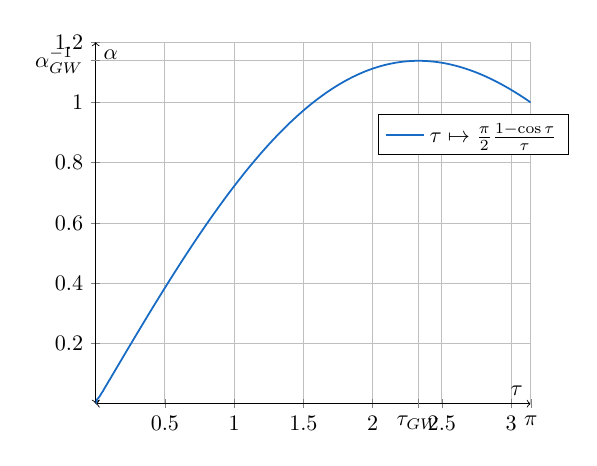
\begin{tikzpicture}[scale=0.8,
    declare function={
    mycos(\t) = cos(180 * \t / pi);
    }
    ]
    \begin{axis}[
        xmin=0,xmax=pi,
        ymin=0,ymax=1.2,
        axis x line=middle,
        axis y line=middle,
        axis line style=<->,
        xlabel={$\tau$},
        ylabel={$\alpha$},
        extra x ticks = {2.3311,pi},
        extra x tick labels = {$\tau_{GW}$, $\pi$},
        extra y ticks = {1/0.878},
        extra y tick labels = {$\alpha_{GW}^{-1}$},
        grid=both,
        width=\textwidth*0.7,
           legend style={at={(0.65,.8)},anchor=north west},
        ]
        \addplot[no marks,myBrightBlue,thick] expression[domain=0:pi,samples=300]{(pi / 2) * (1 - mycos(x)) / x};
        \addlegendentry{$\tau \mapsto \frac{\pi}{2} \frac{1 - \cos \tau}{\tau}$}
        
    \end{axis}
    \end{tikzpicture}
    \caption{Function giving rise to $\alpha_{GW}, \tau_{GW}$.}
    \label{fig:GW}
\end{figure}
Why would $\maxPCSP(K_2, \G_3)$ be easier to approximate than $\maxPCSP(K_2, K_2)$? Consider the Goemans-Williamson algorithm for $\maxPCSP(K_2, K_2)$; the worst-case performance of this algorithm appears in a graph where the embedding into $\R^N$ given by solving the SDP \eqref{eq:sdp} gives all edges an angle of approximately $\tau_{GW}$. Observe that $\tau_{GW} > 2\pi /3$ --- so immediately (cf.~\Cref{lem:noTriangles}) this instance is triangle-free. So, for this instance an algorithm for $\maxPCSP(K_2, \G_3)$ could just return the entire graph! Indeed, in order to create an instance that contains triangles
one needs to introduce shorter edges. This suggests that a hybrid algorithm, that either selects ``long edges'' or some appropriate selection of ``shorter edges''  (still longer than some threshold), should have better performance.
The details can be found in~\Cref{sec:tractability}, while the \NP-hardness part
of~\Cref{thm:main} is proved in~\Cref{sec:hardness}.

\medskip
Our next result is a combination of
the Goemans-Williamson SDP for Max-Cut~\cite{GW95} and a rounding scheme due to Frieze
and Jerrum for Max-3-Cut~\cite{FJ97}.

\begin{restatable}{theorem}{thmktwokthree}\label{thm:k2k3}
$\maxPCSP(K_2, K_3)$ is 1-approximable in polynomial time (in the search version).
\end{restatable}

This algorithm is somewhat similar to the Goemans-Williams algorithm, except
that rather than selecting a uniformly random hyperplane, it selects three
normally distributed vectors, and partitions the vertices according to which
vector they are closest to (where closeness is measured in terms of inner
products). Thus, while this algorithm solves the same SDP as the algorithm
from~\Cref{thm:main}, it rounds the solution differently. This rounding scheme is the same as the rounding scheme of~\cite{FJ97}; it is also very similar to one of the rounding schemes of~\cite{Karger98:jacm}. The details can be
found in~\Cref{sec:23}.

\medskip

The key in proving \NP-hardness in~\Cref{thm:UGCdichotomy} is the following
result, established by generalising the proof of Dinur, Mossel, and
Regev\cite{Dinur09:sicomp} with a multilayered unique games conjecture, in the
style of~\cite{BWZ21}. The details can be found in~\Cref{sec:ugchardness}.

\begin{restatable}{theorem}{thmUGChardness} \label{thm:ugcHardness}
    For every $k\geq 1$ and $\ell \geq 3$, 1-approximation of $\maxPCSP(C_{2k+1},
    K_\ell$) is \NP-hard assuming the \UGC.
\end{restatable}

We now have all tools to prove~\Cref{thm:UGCdichotomy}.

\begin{proof}\textcolor{red}{TOPROVE 0}\end{proof}

We note that our hardness result depends in an essential way on the fact that the input graph can have multiple edges; we equivalently could have allowed non-negative integer weights on the edges. This variant of the problem is most natural when looking at it as a constraint satisfaction problem. It is  interesting to ask what the complexity of $\maxPCSP(K_2, \G_3)$ is if the input graph is  both weightless and without multiple edges.


\section{\texorpdfstring{Approximation of $\maxPCSP(K_2, {\mathfrak{G}}_3)$}{Approximation of maxPCSP(K2,G3)}}
\label{sec:tractability}

In this section, we will prove the tractability part of the following result.

\main*

We will need the following technical lemma.

\begin{lemma}\label{lem:bounds}
    There exist $\alpha, P, Q, \tau \in \R$ with $P + Q = 1, P \geq 0, Q \geq 0$, $\tau \in [2 \pi / 3, \tau_{GW}]$, such that the following hold
\begin{align}
    P \frac{\theta}{\pi} + Q \geq \alpha \frac{1 - \cos\theta}{2} && \theta \in [\tau, \pi]\label{eq:cons1}\\
    P \frac{\phi}{\pi} + Q \frac{\phi}{\pi} \geq \alpha \frac{1 - \cos\phi}{2} && \phi \in [\pi - \tau/2, \tau]\label{eq:cons2}\\
    P \frac{\psi}{\pi} \geq \alpha \frac{1 - \cos \psi}{2} && \psi \in [0, \pi- \tau/2].\label{eq:cons3}
\end{align}
In particular, we can take $\alpha \geq 0.88232, \tau = 2.18746$, $Q = 1 - P$ and
\[
P = \frac{\alpha \pi}{2} \left(\frac{1 - \cos(\pi - \tau / 2)}{\pi - \tau / 2} \right) \approx 0.987535.
\]
\end{lemma}

\begin{proof}\textcolor{red}{TOPROVE 1}\end{proof}

We now prove the desired tractability result.\footnote{We remark in passing that \emph{no} SDP-based algorithm can have performance greater than $8/9 = 0.888\ldots$, since for the triangle $K_3$ the SDP value is $9/4$, yet the largest triangle-free subgraph has weight $2$ (and $2 / (9/4) = 8/9$).}

\begin{theorem}\label{thm:approx}
    $\maxPCSP(K_2, \G_3)$ can be $0.8823$-approximated in polynomial time.
\end{theorem}
\begin{proof}\textcolor{red}{TOPROVE 2}\end{proof}

It is also interesting to consider what the power of our approximation algorithm
is in the \emph{almost satisfiable regime}, i.e.~if an input graph that has a
cut of value $1 - \epsilon$. It turns out that in this case we output a
triangle-free subgraph with $1 - O(\epsilon)$ edges, significantly more than the
$1 - O(\sqrt{\epsilon})$ edges outputted by the Goemans-Williamson
algorithm~\cite{GW95}.
This is not very hard to see, it follows immediately from the fact that our algorithm can choose all edges of angle $> \tau$ immediately.

\begin{theorem}\label{thm:almost}
    The derandomised algorithm from \Cref{thm:approx}, if run on an input graph $G$ with a cut with a  $(1 - \epsilon)$-fraction of edges, produces a triangle-free subgraph with $(1 - O(\epsilon))$-fraction of edges.
\end{theorem}
Indeed, the (extremely loose) analysis below gives us that it returns a triangle-free subgraph with a $(1 - 15\epsilon)$-fraction of edges at least.
\begin{proof}\textcolor{red}{TOPROVE 3}\end{proof}

Interestingly, the non-derandomised algorithm has worse performance! Since it chooses at random between selecting all long edges deterministically and cutting according to the Goemans-Williamson algorithm, the performance degrades to $1 - O(\sqrt{\epsilon})$.

    

\section{\texorpdfstring{Approximation of $\maxPCSP(K_2,K_3)$}{Approximation of maxPCSP(K2,K3)}}
\label{sec:23}

We first introduce some useful notation.
For any predicate $\phi$, we let $[\phi] = 1$ if $\phi$ is true, and $0$ otherwise.

For an event $\phi$ we let $\Pr [\phi]$ be the probability that $\phi$ is true. For a random variable $X$, we let $\mathbb{E}[X]$ denote its expected value. Note that $\mathbb{E}[ [\phi]] = \Pr[\phi]$.
For any two distributions $\mathcal{D}, \mathcal{D}'$ with domains $A, A'$, we let $\mathcal{D} \times \mathcal{D}'$ denote the product distribution, whose domain is $A \times A'$.
For any distribution $\mathcal{D}$ over $\R$ and $a, b \in \R$, the distribution $a\mathcal{D} + b$ is the distribution of $aX + b$ when $X \sim \mathcal{D}$.
We use the standard probability theory abbreviations i.i.d.~(independent and identically distributed) and p.m.f.~(probability mass function).

We introduce a few classic distributions we will need. The uniform distribution $\mathcal{U}(D)$ over a discrete set $D$ is the distribution with p.m.f.~$f : D \to [0, 1]$ given by $f(x) = 1 / |D|$. Note that $\mathcal{U}(D^n)$ is the same as ${\mathcal{U}(D)}^n$, a fact which we will use implicitly. We let $\NBin(n)$ denote a normalised binomial distribution: it is the distribution of $X_1 + \cdots + X_n$, where $X_i \sim \mathcal{U}(\{-1/\sqrt{n}, 1/\sqrt{n}\})$. The domain of this distribution is $\{(-n + 2k) / \sqrt{n} \mid 0 \leq k \leq n\}$, the probability mass function is $(-n + 2k)/\sqrt{n} \mapsto \binom{n}{k} / 2^n$, the expectation is 0, and the variance is 1.
If $\mu, \sigma \in \R$, then we let $\mathcal{N}(\mu, \sigma^2)$ denote the normal distribution with mean $\mu$ and variance $\sigma^2$. Fixing $d$, if $\mathbf{\mu} \in \R^d, \mathbf{\Sigma} \in \R^{d\times d}$, then we let $\mathcal{N}(\mathbf{\mu}, \mathbf{\Sigma})$ denote the multivariate normal distribution with mean $\mathbf{\mu}$ and covariance matrix $\mathbf{\Sigma}$. We let $\mathbf{I}_d$ denote the $d \times d$ identity matrix. Observe that if $\mathbf{x} \sim \mathcal{N}( \mathbf{\mu}, \mathbf{\Sigma})$, where $\mathbf{x} \in \R^d$, then for any matrix $A \in \R^{d' \times d}$ we have that $A \mathbf{x} \sim \mathcal{N}(A \mathbf{\mu}, A \mathbf{\Sigma} A^T)$. Furthermore if $\mathbf{x} \sim \mathcal{N}(\mathbf{\mu}, \mathbf{\Sigma})$ with $\mathbf{\Sigma}$ positive semidefinite, then by finding the Cholesky decomposition $\mathbf{\Sigma} = \mathbf{A} \mathbf{A}^T$, where $\mathbf{A} \in \R^{d \times d}$, we find that $\vx$ is identically distributed to $\mathbf{A} \vx' + \mathbf{\mu}$, where $\vx' \sim \mathcal{N}(\mathbf{0}, \mathbf{I}_d)$.

Our goal is to prove the following result.

\thmktwokthree*

Our proof will be split into three parts: First we prove some technical bounds which we will need. Next, we provide a randomised algorithm. Finally, we derandomise the algorithm.

\paragraph{Technical bounds.} For the proof, we will need a technical lemma,
stated as~\Cref{lem:prExpr} below. The proof of~\Cref{lem:prExpr} is an application of the following result of Cheng.

\begin{theorem}[{\cite{Cheng68}\cite[Equation (2.18)]{Cheng69}}]\label{thm:cheng}
Suppose $\mathbf{u} = (u_1, u_2, u_3, u_4) \sim \mathcal{N}(\mathbf{0}, \mathbf{\Sigma})$ are drawn from a quadrivariate normal distribution with mean zero and covariance matrix
\[
\mathbf{\Sigma} =
\begin{pmatrix}
   1 & a & b & ab \\
   a & 1 & ab & b \\
   b & ab & 1 & a \\
   ab & b & a & 1 \\
\end{pmatrix},
\]
where $a, b \in [-1, 1]$. Then $\Pr_{\mathbf{u}}[u_1 \geq 0, u_2 \geq 0, u_3 \geq 0, u_4 \geq 0]$ is 
\[
\frac{1}{16} + \frac{\arcsin a + \arcsin b + \arcsin ab}{4\pi} + \frac{{(\arcsin a)}^2 + {(\arcsin b)}^2 - {(\arcsin ab)}^2}{4\pi^2}.
\]
\end{theorem}

\begin{lemma}\label{lem:prExpr}
Fix $\alpha, \beta \in \mathbb{R}$ such that $\alpha^2 + \beta^2 = 1$. Suppose $x_1, x_2, x_3, y_1, y_2, y_3 \sim \mathcal{N}(0, 1)$ i.e.~they are i.i.d.~standard normal variables. The probability that
\begin{align*}
x_1 & \geq x_2 \\
x_1 & \geq x_3 \\
\alpha x_1 + \beta y_1 & \geq  \alpha x_2 + \beta y_2 \\
\alpha x_1 + \beta y_1 & \geq  \alpha x_3 + \beta y_3 \\
\end{align*}
is precisely
\[
P(\alpha) = 
\frac{1}{9}
+ \frac{\arcsin \alpha + \arcsin \frac{\alpha}{2}}{4\pi} 
+ \frac{
{(\arcsin \alpha)}^2-
{(\arcsin \frac{\alpha}{2})}^2
}{4\pi^2}.
\]
\end{lemma}
\begin{proof}\textcolor{red}{TOPROVE 4}\end{proof}

We will need a bound on the $P(\alpha)$ function from~\Cref{lem:prExpr}.

\begin{lemma}\label{lem:ineq}
    For $-1 \leq \alpha \leq -1$, $1 - 3P(\alpha) \geq \frac{1 - \alpha}{2}$.
\end{lemma}
\begin{figure}
\begin{center}
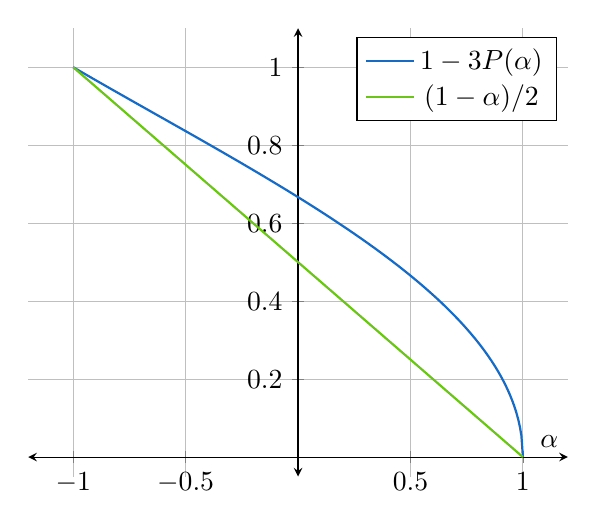
\begin{tikzpicture}[>=stealth]
    \begin{axis}[
        xmin=-1.2,xmax=1.2,
        ymin=-0.05,ymax=1.1,
        axis x line=middle,
        axis y line=middle,
        axis line style=<->,
        xlabel={$\alpha$},
        grid=both,
        ]
        \addplot[name path=a, no marks,myBrightBlue,thick] expression[domain=-1:1,samples=300]{1 - 3*(1/9 + (rad(asin(x)) + rad(asin(x/2)))/(4*pi) + (rad(asin(x))^2 - rad(asin(x/2))^2)/(4*pi*pi))};
        \addlegendentry{$1 - 3P(\alpha)$}
        \addplot[name path=b, no marks,myBrightGreen,thick] expression[domain=-1:1,samples=100]{(1-x)/2};
        \addlegendentry{$(1 - \alpha)/2$}
    \end{axis}
\end{tikzpicture}
\end{center}
\caption{Plot of expressions from~\Cref{lem:ineq}.}\label{fig:plots}
\end{figure}
The functions involved are shown in~\Cref{fig:plots}.
\begin{proof}\textcolor{red}{TOPROVE 5}\end{proof}

\paragraph{Randomised algorithm.} We first provide a randomised version of our algorithm, accurate up to some $\epsilon$.

\begin{theorem}[Randomised version of~\Cref{thm:k2k3}]
    There exists a randomised algorithm which, given a graph $G = (V, E)$ that has a cut with $\rho$ edges and an accuracy parameter $\epsilon$, finds a 3-colouring of $G$ that satisfies $\rho-\epsilon$ edges in expectation, in polynomial time with respect to the size of $G$ and $\log(1 / \epsilon)$.
\end{theorem}

\begin{proof}\textcolor{red}{TOPROVE 6}\end{proof}


\paragraph{Derandomised algorithm.}
We will now show how to derandomise our algorithm, using
the method of conditional expectations, which was also used by Mahajan
and Ramesh~\cite{Mahajan99:sicomp}. The approach of Bhargava and
Kosaraju~\cite{BK05} derandomises conditional probabilities by an approximation
of normal distributions via polynomials; we approximate simply just with a
scaled bionomial distribution. We believe that the results of the literature are sufficient to prove the derandomisation theorem we need (which crucially needs to work for our 1-approximation setting); however we propose a simpler derandomisation method that we believe will be easier to apply in general. (Indeed, our method avoids integration alltogether.) There is an interesting duality between our approach and that of Mahajan and Ramesh: we discretise the normal distribution, whereas they discretise the SDP vectors.
    

Our goal will be the following general derandomisation theorem.

\begin{theorem}\label{thm:derandGaussian}
    Fix a constant $d$. There exists an algorithm that does the following. Suppose we are given $n, m \in \mathbb{N}$, $\vx_{ij} \in \mathbb{R}^n$ and $y_{ij}, \varepsilon \in \mathbb{R}$ for all $i \in [m], j \in [d]$. Suppose $\va = (a_1, \ldots, a_n) \sim \mathcal{N}(\mathbf{0}, \mathbf{I}_n)$ and that
    \[
    \sum_{i = 1}^m \Pr_{\va}\left[ \bigwedge_{j = 1}^d \vx_{ij} \cdot \va > y_{ij} \right] \geq \rho
    \]
    for some $\rho \in \mathbb{R}$. Then the algorithm computes some particular $\va^* = (a_1^*, \ldots, a_n^*) \in \mathbb{R}^n$ such that
    \[
    \sum_{i =1 }^m \left[ \bigwedge_{j = 1}^d \vx_{ij} \cdot \va^* > y_{ij} \right] \geq \rho - \varepsilon,
    \]
    in polynomial time with respect to $n, m, 1/\varepsilon$.
\end{theorem}

To facilitate the proof of~\Cref{thm:derandGaussian}, we will need a multidimensional version of the Berry-Esseen theorem. We will use the following version with explicit constants, due to Rai\v{c}~\cite{Raic19}.

\begin{theorem}[{\cite[Theorem~1.1]{Raic19}}]\label{thm:BE}
Suppose $\mathbf{t}_1, \ldots, \mathbf{t}_N \in \mathbb{R}^d$ are independent random variables with mean zero, such that the sum of their covariance matrices is $\mathbf{I}_d$. Let $\mathbf{s} = \mathbf{t}_1 + \cdots + \mathbf{t}_N$. Suppose $\va \sim \mathcal{N}(\mathbf{0}, \mathbf{I}_d)$, and let $C \subseteq \mathbb{R}^d$ be convex and measurable. Then
\[
| \Pr_{\mathbf{s}}[\mathbf{s} \in C] - \Pr_{\va}[\va \in C] | \leq \left(42\sqrt[4]{d} + 16\right) \sum_{i = 1}^N \mathbf{E} \left[ || \mathbf{t}_i ||^3 \right].
\]
\end{theorem}

The following is an easy and well-known corollary of~\Cref{thm:BE}: We can approximate a multivariate normal distribution with binomial distributions. For completeness, we provide a proof.

\begin{corollary}\label{corr:appliedBerryEsseen}
Let $d \in \mathbb{N}$ be a constant and take $\varepsilon \in (0, 1)$. Take
\begin{equation}\label{eq:defN}
N = N_\varepsilon \geq {\left(\frac{42 d^{7/4} +16 d^{3/2} }{\varepsilon}\right)}^2 = \frac{\xi_d}{\varepsilon^2},
\end{equation}
where $\xi_d = O(d^{7/2})$ depends only on $d$. Suppose
$s_1, \ldots, s_N \sim \NBin(N)$ are i.i.d., and let $\mathbf{s} = (s_1, \ldots, s_d)$.
 Let $\va \sim \mathcal{N}(\mathbf{0}, \mathbf{I}_d)$. Then for all convex measurable sets $C \subseteq \mathbb{R}^d$ we have
\[
| \Pr_{\mathbf{s}}[ \mathbf{s} \in C] - \Pr_{\va}[\va \in C] | \leq \varepsilon.
\]
\end{corollary}
\begin{proof}\textcolor{red}{TOPROVE 7}\end{proof}

\begin{theorem}\label{thm:stepApprox}
    Fix a constant $d$, and take $\vx_{1}, \ldots, \vx_d \in \mathbb{R}^n, y_1, \ldots, y_d \in \mathbb{R}, z_1, \ldots, z_d \in \mathbb{R}, \epsilon \in \mathbb{R}$. Consider the function
    \[
    p(t) = \Pr_{\va \sim \mathcal{N}(\mathbf{0}, \mathbf{I}_n)}\left[\bigwedge_{i=1}^d \vx_{i} \cdot \va + z_i t > y_i \right].
    \]
    There exists a step function $\widehat{p}$ with $\poly(1/\epsilon)$ steps, where the steps and the values at those steps are computable in polynomial time with respect to $1 / \epsilon$
    and $n$, such that $| \widehat{p}(t) - p(t)| \leq \epsilon$ for all $t \in \mathbb{R}$.
\end{theorem}
\begin{proof}\textcolor{red}{TOPROVE 8}\end{proof}

\begin{proof}\textcolor{red}{TOPROVE 9}\end{proof}

This is enough to derandomise our algorithm.

\begin{proof}\textcolor{red}{TOPROVE 10}\end{proof}


\section{\texorpdfstring{Hardness of $\maxPCSP(K_2, \G_3)$}{Hardness of maxPCSP(K2,G3)}}
\label{sec:hardness}

In this section, we will prove the hardness part of the following result.

\main*

Our general strategy will be to gadget reduce from the 3-bit PCP of H{\aa}stad ~\cite{Hastad01}, similarly to~\cite{Trevisan00:sicomp} or~\cite{BGS:98}. The main difficulty comes in from the fact that it is not possible to ``negate'' variables in an obvious way, since ``negation'' is not globally preserved by the property of being triangle-free, as opposed to that of being bipartite. Some mild complications will be forced by this. Recall first the definition of exactly-3 linear equations.

\begin{definition}
    In the problem $\elin_\delta$, one is given a system of mod-2 linear
    equations with exactly 3 variables per equation; i.e.~$x + y + z \equiv 0
    \bmod 2$ or $x + y + z \equiv 1 \bmod 2$. If it is possible to
    simultaneously solve a $1 - \delta$ fraction of all the equations, one must
    answer \textsc{Yes}; otherwise, if it is not even possible to simultaneously solve a $\frac{1}{2} + \delta$ fraction of the equations, one must answer \textsc{No}.
\end{definition}

\begin{theorem}[\cite{Hastad01}]
    For every small enough $\delta$, the problem $\elin_\delta$ is \NP-hard.
\end{theorem}

To deal with our negation problems, we will need a ``balanced'' version of this problem.

\begin{definition}
    In the problem $\belin_\delta$, one is given a system of mod-2 linear equations with exactly 3 variables per equation; i.e.~$x + y + z \equiv 0 \bmod 2$ or $x + y + z \equiv 1 \bmod 2$. Furthermore, the number of equations of the two types is equal. 
    A \emph{balanced solution} to such a system of equations is one that satisfies exactly as many equations of form $x + y + z \equiv 0 \bmod 2$ as those of form $ x + y + z \equiv 1 \bmod 2$.
    
    If it is possible to find a balanced solution that satisfies a $1 - \delta$ fraction of all the equations, one must answer \textsc{Yes}; otherwise, it if is not even possible to find any (\emph{possibly even unbalanced}) solution that satisfies a $\frac{1}{2} + \delta$ fraction of the equations, one must answer \textsc{No}.
\end{definition}

We believe 
that~\cite{Hastad01} proves, without being explicit about it, \NP-hardness of $\belin_\delta$, although it is not straightforward to see it from the proof in~\cite{Hastad01}. For completeness, we provide a simple, self-contained reduction.

\begin{lemma}\label{lem:source}
    For every small enough $\delta$, the problem $\belin_\delta$ is \NP-hard.
\end{lemma}

\begin{proof}\textcolor{red}{TOPROVE 11}\end{proof}


We now define the notion of ``gadget'' that we will need for this particular reduction. This is along the same lines as~\cite{BGS:98,Trevisan00:sicomp}, but (i) generalised to deal with promise problems and (ii) specialised to our particular promise problem.

For the following, if $G = (V, E)$ is any bipartite graph, and $V' \subseteq V$, then we say that a function $c : V' \to \{ 0, 1 \}$ is compatible with $G$ if it is possible to extend $c$ into a 2-colouring of $G$.

\begin{definition}\label{def:gadget}
    A gadget with performance $\alpha \in \N$ and parity $p \in \{0, 1\}$ is a graph $G = (V, E)$, with $0, x, y, z \in V$, where the following hold.
    \begin{enumerate}
        \item\label{item:soundness} For any function $c : \{ 0, x, y, z \} \to \{0, 1\}$ such that $c(0) + c(x) + c(y) + c(z) \equiv p \bmod 2$, there exists a bipartite subgraph $H$ of $G$ with $\alpha$ edges, such that $c$ is compatible with $H$.
        \item\label{item:completenes1} Any triangle-free subgraph of $G$ has at most $\alpha$ edges.
        \item\label{item:completenes2} Every triangle-free subgraph $H$ of $G$ with strictly more than $\alpha-1$ edges puts $0, x, y, z$ in the same connected component $C$, and the distance from $0$ to $x, y, z$ respectively is at most 2. Furthermore $C$ is bipartite, and for any $c : \{0, x, y, z\} \to \{0, 1\}$ that is compatible with $C$, we have that $c(0) + c(x) + c(y) + c(z) \equiv p \bmod 2$.
    \end{enumerate}
\end{definition}

\begin{lemma}\label{lem:bins}
    Suppose we have $n$ containers with capacities $c_1, \ldots, c_n \geq 0$. Suppose we distribute a volume of $c_1 + \cdots + c_n - n + a$ among the containers, distributing $v_i \leq c_i$ volume to container $i$. Then the number of containers $i$ for which $v_i > c_i - 1$ is at least $a$.
\end{lemma}
\begin{proof}\textcolor{red}{TOPROVE 12}\end{proof}

The next theorem encodes our reduction from 
the 3-bit PCP of~\cite{Hastad01} to $\maxPCSP(K_2, \G_3)$. This reduction is standard, needing only some care to deal with the fact that the triangle-free graph selected in the soundness case must be ``connected enough''.

\begin{theorem}
    Suppose that for $i \in \{0, 1\}$ there exist gadgets $G_i$ with performance $\alpha_i$ and parity $i$. Then it is \NP-hard to approximate $\maxPCSP(K_2, \G_3)$  with approximation ratio $1 - 1 / (\alpha_0 + \alpha_1) + \epsilon$.
\end{theorem}
\begin{proof}\textcolor{red}{TOPROVE 13}\end{proof}
 
We now exhibit the gadgets. The first gadget is identical to a gadget of Bellare, Goldreich and Sudan~\cite{BGS:98} (although our analysis is slightly more complicated). In~\cite{BGS:98}, this gadget is called ``PC-CUT'', defined immediately before~\cite[Claim~4.17]{BGS:98}. The second gadget is a generalisation of the first. Recall that the gadgets of~\cite{BGS:98} were improved in~\cite{Trevisan00:sicomp}, and indeed the results of~\cite{Trevisan00:sicomp} indicate a generic method to find optimal gadgets for finite-domain CSPs. We do not believe this approach directly applies to our case because the property of being triangle-free is not captured by any finite CSP template (indeed, $\G_3$ is infinite, and any homomorphism-equivalent structure must also be).

We will write our gadgets as graphs with non-negative integer weights for simplicity of presentation. These gadgets can then be implemented by adding edges multiple times.



\begin{lemma}
    There exists a gadget with performance 9 and parity 1.
\end{lemma}
\begin{proof}\textcolor{red}{TOPROVE 14}\end{proof}

\begin{lemma}
    There exists a gadget with performance 17 and parity 0.
\end{lemma}
\begin{proof}\textcolor{red}{TOPROVE 15}\end{proof}

\newpage

\section{\texorpdfstring{Hardness of $\maxPCSP(C_{2k+1}, K_\ell)$}{Hardness of maxPCSP(C2k+1, Kl)}}
\label{sec:ugchardness}

In this section, we will prove the following result.

\thmUGChardness*

The proof is a generalisation of the proof
in~\cite{Dinur09:sicomp} that establishes the \NP-hardness of \emph{almost
3-colouring} (i.e.~given an $n$ vertex graph $G$, output \textsc{Yes} if $G$ has
a 3-colourable $(1 - \epsilon)n$ vertex-induced subgraph, and \textsc{No} if $G$
does not even have an independent set with more than $\epsilon n$ vertices), assuming the \UGC.
We will need, unlike~\cite{Dinur09:sicomp}, a
\emph{multilayered unique games conjecture}, in the style of~\cite{BWZ21}. We
first set up the necessary ingredients. The proof is based on \emph{Markov-chain noise operators} --- the one we will use is intimately related to $C_{2k + 1}$.

\begin{definition}
    Define $M_{n}$ to be the matrix which has $\frac{1}{2}$ at position $(i, j)$ if and only if $|i - j| \equiv 1 \bmod n$. I.e.~$M_{n}$ is the \emph{circulant matrix} given by the vector $(0, \frac{1}{2}, 0, \ldots, 0, \frac{1}{2})$, of length $n$. Note that $M_{n}$ is a Markov chain on $[n]$, and $(i, j)$ has nonzero transition probability if and only if $(i, j)$ is an edge of $C_{n}$.
\end{definition}

\begin{lemma}
    The uniform distribution is the stationary distribution of $M_{n}$.
\end{lemma}
\begin{proof}\textcolor{red}{TOPROVE 16}\end{proof}

\begin{lemma}
    Let $\omega$ be the $n$-th root of unity. The eigenvalues of $M_{n}$ are $\cos(2k\pi / n)$ for $k = 0, \ldots, n - 1$. In particular, if $n$ is odd then exactly one eigenvalue has absolute value 1 and the rest have absolute value at most $\cos(1 - \pi/n) < 1$.\footnotemark
\end{lemma}
\footnotetext{This would \emph{not} be true if $n$ were even --- there would be two eigenvalues with absolute value 1, namely $\pm 1$, taking $k = 0$ and $k = n / 2$.}
\begin{proof}\textcolor{red}{TOPROVE 17}\end{proof}

These are the key properties needed to apply the theory of \cite{Dinur09:sicomp}. We will need a multi-layered Unique Games Conjecture, which we now state.

\begin{definition}\label{def:layered}
    An $\ell$-layered unique label-cover instance consists of a set of variables
    $X_1, \ldots, X_\ell$, a domain $[D]$, and a multiset of constraints. Each
    constraint consists of $\ell$ variables $(x_1, \ldots, x_\ell) \in X_1
    \times \cdots \times X_\ell$, together with a family of permutations
    $\pi_{ij}$ on $[D]$ for $1 \leq i < j \leq \ell$, such that $\pi_{ik} =
    \pi_{jk} \circ \pi_{ij}$. A solution is an assignment $c : (X_1  \cup \ldots
    \cup X_\ell) \to [D]$. The assignment $c$ \emph{strongly satisfies} a
    constraint given by $(x_1, \ldots, x_{\ell})$ and $(\pi_{ij})_{1 \leq i < j
    \leq \ell}$ if $\pi_{ij}(c(x_i)) = c(x_j)$ \emph{for all $1 \leq i < j \leq
    \ell$}. The assignment $c$ \emph{weakly satisfies} this same constraint if
    $\pi_{ij}(c(x_i)) = c(x_j)$ \emph{for at least one pair $1 \leq i < j \leq
    \ell$}. The strong value of an instance is the maximum fraction of
    constraints that can be simultaneously strongly satisfied by some
    assignment; the weak value is given by the maximum fraction of constraints
    that can be simultaneously weakly satisfied by some assignment.
\end{definition}

Note that for $\ell = 2$, weak satisfaction and strong satisfaction (and hence weak and strong values) coincide. Hence for $\ell = 2$ we drop the weak/strong distinction.

\begin{conjecture}[\UGC~\cite{Khot02stoc}]\label{conj:UGC}
For every $\epsilon$ there exists $D$ such that, given a 2-layered unique label-cover instance with domain $[D]$, it is \NP-hard to distinguish if the value is at least $1 - \epsilon$ or not even $\epsilon$.
\end{conjecture}

We will show that \Cref{conj:UGC} implies the following conjecture. Our proof
closely follows~\cite{BWZ21}, which in turn builds on~\cite{DinurGKR05}, but is generalised to deal with imperfect completeness.

\begin{conjecture}[Multilayered UGC]\label{conj:mulUGC}
For every $\epsilon, \ell \geq 2$ there exists some $D$ such that, given an $\ell$-layered unique label-cover instance with domain $[D]$, it is \NP-hard to distinguish if the strong value is at least $1 - \epsilon$, or if the weak value is not even $\epsilon$.
\end{conjecture}

\begin{proof}\textcolor{red}{TOPROVE 18}\end{proof}

The proof of~\Cref{thm:ugcHardness} will be based on the \emph{long code
construction}~\cite{BGS:98}. We will now describe the building blocks of our reduction.

\begin{definition}
    Fix $k, \ell, D$. A \emph{cloud} of vertices, denoted by $\vec{f}$, is a set of vertices $f(a_1, \ldots, a_D)$ for $a_1, \ldots, a_D \in [2k + 1]$. For $\ell$ clouds of variables $\vec{f}_1, \ldots, \vec{f}_\ell$ and a family of permutations $\pi_{ij} : [D] \to [D]$ for $1 \leq i < j \leq \ell$ as in \Cref{def:layered}, we define the set of edges $E_\pi(\vec{f}_1, \ldots, \vec{f}_\ell)$ as follows: for every $1 \leq i < j \leq \ell$, $a_1, \ldots, a_D, b_1, \ldots, b_D \in [2k + 1]$ and for which $a_t, b_t$ differ by $\pm 1$ modulo $2k + 1$, we include the edge $f_i(a_{\pi_{ij}(1)}, \ldots, a_{\pi_{ij}(D)}) - f_j(b_1, \ldots, b_D)$.
\end{definition}

The following is the key theorem from~\cite{Dinur09:sicomp} that we will use. We will define some notions, however we refer to~\cite{Dinur09:sicomp} for a full treatment.

\begin{definition}
    For a symmetric Markov operator $T$ on $[q]$, and letting $f, g : [q]^n \to \mathbb{R}$, the value $\langle f, T^{\otimes n} g \rangle$ has the following interpretation. Let $x \in [q]^n$ be distributed uniformly at random, and let $y \in [q]^n$ be such that $y_i$ is distributed according to the transition probabilities in $T$ starting at $x_i$. Then $\langle f, T^{\otimes n} g \rangle$ is the expected value of $f(x) g(y)$.

    The quantity $\langle F_\mu, U_\rho(1 - F_{1 - \nu})\rangle_\gamma$, which we also denote by $\Gamma_\rho(\mu, \nu)$, has the following interpretation. Let $x, y$ be two normally distributed variables with mean 0, variance 1 and covariance $\rho$. Then this value is the probability that $x \leq \Phi^{-1}(\mu), y \geq \Phi^{-1}(1 - \nu)$, where $\Phi$ is the cumulative distribution function of the normal distribution. Essentially, this value is nondecreasing in both $\mu$ and $\nu$.

    For a function $f : [q]^n \to \mathbb{R}$, the value $I_i^{\leq t}(f)$ is the \emph{low-degree influence} of coordinate $i$ in $f$. In particular, if $f(x) \in [0, 1]$, it can be shown that $\sum_{i = 1}^n I_i^{\leq t}(f) \leq t$ and $I_i^{\leq t}(f) \geq 0$. Furthermore, the influence of a coordinate is defined compatibly with permuting coordinates i.e.~if the influence of coordinate $i$ is $x$, and we permute the coordinates of $f$ so as to move $i$ to position $j$, yielding a function $g$, then the influence of $j$ in $g$ is still $x$.
\end{definition}

\begin{theorem}[\cite{Dinur09:sicomp}]\label{thm:dinur_thm}
    Fix $q$ and let $T$ be a symmetric Markov operator on $[q]$ with spectral radius $\rho < 1$ (by spectral radius we mean the second largest eigenvalue of $T$ in absolute value). Then for any $\epsilon > 0$ there exist $\delta > 0$ and $t \in \mathbb{N}$ so that if $f, g : [q]^n \to [0, 1]$ are two functions with
    \[
    \min(I_i^{\leq t}(f), I_i^{\leq t}(g)) < \delta,
    \]
    for all $i$, then
    \[
    \langle f, T^{\otimes n} g\rangle \geq \langle F_\mu, U_\rho (1 - F_{1 - \nu})\rangle_\gamma - 
    \epsilon,
    \]
    where $\mu = E[f], \nu = E[g]$.
\end{theorem}

Similarly to \cite{Dinur09:sicomp}, we will use this in the contrapositive, in particular in the following form.

\begin{corollary}\label{cor:technical}
    Fix $q$ and let $T$ be a symmetric Markov operator on $[q]$ with spectral radius $\rho < 1$. For every $\epsilon$ there exists $\delta > 0$ and $t \in \mathbb{N}$ so that, if $f, g : [q]^n \to [0, 1]$ are two functions with $E[f] \geq \epsilon, E[g] \geq \epsilon$ and $\langle f, T^{\otimes n} g\rangle \leq \delta$, then there exists $i \in [n]$ so that $I_i^{\leq t}(f) \geq \delta$ and $I_i^{\leq t}(g) \geq \delta$.
\end{corollary}
\begin{proof}\textcolor{red}{TOPROVE 19}\end{proof}

\begin{lemma}\label{lem:technical}
    There exists $s, \delta$ which depend only on $k, \ell$ so that the following holds for any $D$.
    
    Consider an $\ell$-colouring $\vec{f} \to [\ell]$ of the cloud of vertices $\vec{f}$. We denote the vertex $f(a_1, \ldots, a_D)$ receiving colour $c$ by $f(a_1, \ldots, a_D) = c$. There exists a way to assign any such cloud a subset $I(\vec{f})$ of $[D]$ of size $s$ such that the following holds.

    Consider any $\ell + 1$ clouds $\vec{f}_1, \ldots, \vec{f}_{\ell + 1}$ and a family of permutations $\pi_{ij}$ as in \Cref{def:layered}. Suppose that these vertices are $\ell$-coloured, and that the $\ell$-colouring satisfies a $(1 - \delta)$-fraction of the edges in $E_\pi(\vec{f}_1, \ldots, \vec{f}_{\ell + 1})$. Then there exists $1 \leq i < j \leq \ell + 1$ such that $\pi_{ij}(I(\vec{f}_i)) \cap I(\vec{f}_j) \neq \emptyset$.
\end{lemma}
\begin{proof}\textcolor{red}{TOPROVE 20}\end{proof}
 
\begin{theorem}
    \Cref{conj:mulUGC} implies \Cref{thm:ugcHardness}.
\end{theorem}
\begin{proof}\textcolor{red}{TOPROVE 21}\end{proof}

\section*{Acknowledgements}

We thank Jakub Opr\v{s}al, who asked us about the complexity of $\maxPCSP$s for
graphs beyond cliques, and for useful discussions. We also thank Pravesh Kothari
for asking us about the performance of our maximum bipartite vs.~triangle-free
subgraph algorithm in the $1 - \epsilon$ regime, which led to~\Cref{thm:almost}.

{
\bibliography{nz}
\bibliographystyle{alphaurl}
}

\end{document}
